% Chương 2

\chapter{CƠ SỞ LÝ THUYẾT}

\label{Chapter2}

%----------------------------------------------------------------------------------------

\section{Tổng quan về khối dữ liệu 3D trong Y khoa}

Nếu như trong ảnh 2D, đơn vị cơ bản cấu tạo nên bức ảnh là Điểm ảnh (Pixel -- Picture Element), thì trong không gian 3D, phần tử cơ bản được gọi là \textbf{Điểm thể tích (Voxel -- Volume Element)}. Mỗi voxel trong khối dữ liệu chứa một giá trị cường độ sáng tương ứng với mật độ quang học hoặc cấu trúc vật lý của mô tại tọa độ không gian $(x, y, z)$ đó~\cite{gonzalez2018digital}.

Khối dữ liệu 3D thực chất là một tập hợp của hàng trăm đến hàng ngàn lát cắt 2D (Slices) được xếp chồng lên nhau dọc theo trục $Z$. Do kích thước dữ liệu khổng lồ (thường lên đến hàng tỷ voxel), việc truy xuất và xử lý khối dữ liệu này đòi hỏi tài nguyên bộ nhớ lớn và năng lực tính toán tốc độ cao.

%----------------------------------------------------------------------------------------

\section{Kiến trúc Lập trình song song CUDA}

CUDA (Compute Unified Device Architecture) là một nền tảng tính toán song song và mô hình lập trình do NVIDIA phát triển, cho phép tận dụng tối đa sức mạnh của các Bộ xử lý đồ họa (GPU) để giải quyết các bài toán tính toán phức tạp~\cite{nvidia_cuda_guide}.

\begin{figure}[h]
    \centering
    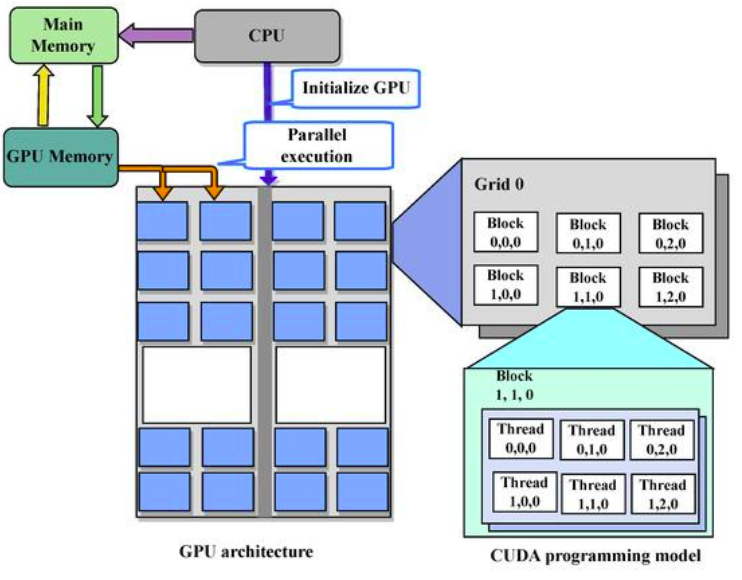
\includegraphics[height=8cm, keepaspectratio]{Figures/Chapter/1.png}
    \caption{Mô hình lập trình CUDA}
    \label{fix:chapter1_1}
\end{figure}

Mô hình lập trình CUDA phân chia hệ thống thành hai phần chính:

\begin{itemize}
    \item \textbf{Host (Máy chủ):} Bao gồm CPU và bộ nhớ chính (RAM), đóng vai trò điều khiển luồng chương trình, cấu hình thông số và khởi tạo dữ liệu.
    \item \textbf{Device (Thiết bị):} Bao gồm GPU và bộ nhớ video (VRAM), chuyên đảm nhận các tác vụ tính toán chuyên sâu mang tính lặp đi lặp lại.
\end{itemize}

\textbf{Cấu trúc phân cấp luồng (Thread Hierarchy):} Để quản lý hàng chục ngàn phép tính diễn ra cùng lúc, CUDA tổ chức các luồng thực thi theo ba cấp độ:

\begin{enumerate}
    \item \textbf{Thread (Luồng):} Đơn vị tính toán nhỏ nhất. Mỗi Thread thường chịu trách nhiệm tính toán cho đúng một điểm ảnh (pixel/voxel).
    \item \textbf{Block (Khối):} Tập hợp của nhiều Thread. Các Thread trong cùng một Block có thể giao tiếp và chia sẻ dữ liệu với nhau thông qua bộ nhớ chung (Shared Memory).
    \item \textbf{Grid (Lưới):} Tập hợp của nhiều Block. Kích thước của Grid được thiết kế để bao phủ toàn bộ không gian của khối dữ liệu cần xử lý.
\end{enumerate}

%----------------------------------------------------------------------------------------

\section{Cơ sở thuật toán nhánh phân tích mạch máu (Vessel Analysis)}

\subsection{Thuật toán chiếu ảnh cường độ tối đa (MIP)}

MIP (Maximum Intensity Projection) là phương pháp nén khối dữ liệu 3D thành bản đồ 2D~\cite{defined_mip}. Thuật toán mô phỏng việc chiếu các tia sáng dọc theo trục $Z$ của khối. Trên mỗi đường truyền của tia từ mặt trên xuống mặt đáy, thuật toán sẽ lấy giá trị voxel có cường độ sáng lớn nhất để chiếu lên mặt phẳng 2D:
\begin{equation}
    I_{MIP}(x,y) = \max_{z=0}^{D-1} V(x, y, z)
    \label{eq:mip}
\end{equation}
trong đó $V(x, y, z)$ là giá trị voxel tại tọa độ $(x, y, z)$ và $D$ là chiều sâu của khối dữ liệu.

\begin{figure}[h]
    \centering
    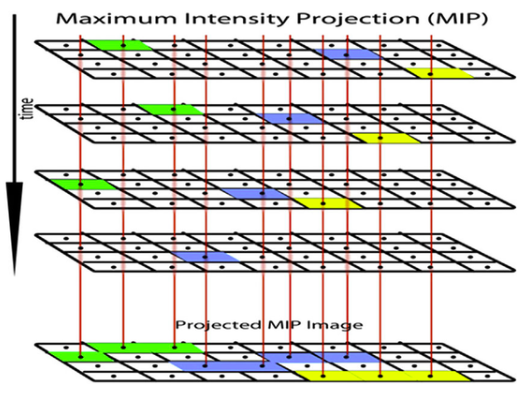
\includegraphics[height=8cm, keepaspectratio]{Figures/Chapter/2.png}
    \caption{Mô hình lập trình CUDA}
    \label{fix:chapter1_2}
\end{figure}

Do mạch máu thường có mức độ phản xạ quang học sáng hơn so với mô nền, thuật toán MIP giúp trích xuất toàn bộ mạng lưới mạch máu ẩn bên trong lớp da lên một bức ảnh bề mặt duy nhất.

\subsection{Bộ lọc trung bình (Mean Filter)}

Trong quá trình thu nhận tín hiệu từ các thiết bị chụp cắt lớp (như CT, MRI hay OCT), hình ảnh thường bị suy giảm chất lượng do sự xuất hiện của các loại nhiễu ngẫu nhiên, đặc biệt là nhiễu hạt (\textit{speckle noise}) và nhiễu Gaussian. Để loại bỏ các thành phần nhiễu này và cải thiện tỷ số tín hiệu trên nhiễu (SNR), một bộ lọc không gian tuyến tính — cụ thể là bộ lọc trung bình (\textit{Mean Blur}) với kích thước cửa sổ (kernel) $3 \times 3$ — được áp dụng lên từng điểm ảnh.

Giá trị của điểm ảnh sau khi làm mịn tại tọa độ $(x, y)$ được xác định bằng trung bình cộng giá trị của chính nó và các điểm ảnh lân cận trong phạm vi cửa sổ lọc, tuân theo công thức toán học sau:

\begin{equation}
I_{\text{blur}}(x, y) = \frac{1}{9} \sum_{i=-1}^{1} \sum_{j=-1}^{1} I(x + i, y + j)
\label{eq:mean_filter}
\end{equation}

Trong đó:
\begin{itemize}
    \item $I(x, y)$ là giá trị cường độ sáng của điểm ảnh gốc tại tọa độ $(x, y)$.
    \item $I_{\text{blur}}(x, y)$ là giá trị cường độ sáng của điểm ảnh sau khi đã áp dụng bộ lọc trung bình.
    \item $i$ và $j$ là các chỉ số dịch chuyển trong không gian hai chiều của cửa sổ lọc kích thước $3 \times 3$.
\end{itemize}

Về mặt hiệu quả xử lý, kỹ thuật lọc không gian này đóng vai trò quan trọng trong việc làm mịn vùng nền mô xung quanh, giảm thiểu các biến động tần số cao do nhiễu gây ra. Đồng thời, quá trình làm mịn cấu trúc này còn hỗ trợ kết nối các phân đoạn mạch máu bị đứt gãy cục bộ do suy hao tín hiệu, tạo điều kiện thuận lợi cho các bước phân đoạn ảnh (\textit{segmentation}) và trích xuất hình thái mạch máu tiếp theo.

\subsection{Thuật toán phân ngưỡng nhị phân (Thresholding)}

Sau giai đoạn làm mịn và giảm nhiễu, thuật toán phân ngưỡng nhị phân (\textit{Binary Thresholding}) được áp dụng như một bước tiền xử lý quyết định nhằm tách biệt đối tượng quan tâm (mạch máu, tổn thương) ra khỏi vùng nền cấu trúc mô. Bản chất của kỹ thuật này là chuyển đổi một ảnh xám (\textit{grayscale image}) có dải giá trị liên tục thành một ảnh nhị phân (\textit{binary image}) chỉ bao gồm hai màu đen và trắng thuần túy.

Quá trình chuyển đổi được thực hiện bằng cách so sánh cường độ sáng của từng điểm ảnh $I(x, y)$ tại vị trí tọa độ $(x, y)$ với một giá trị ngưỡng cường độ cố định $T$ (chọn trước dựa trên thực nghiệm hoặc giải thuật tối ưu, ví dụ: $T = 140$). Hàm toán học phân ngưỡng được định nghĩa như sau:

\begin{equation}
I_{\text{binary}}(x, y) = 
\begin{cases} 
255 & \text{nếu } I(x, y) > T \\ 
0 & \text{nếu } I(x, y) \le T 
\end{cases}
\label{eq:thresholding}
\end{equation}

Trong đó:
\begin{itemize}
    \item $I(x, y)$ là giá trị mức xám gốc của điểm ảnh tại tọa độ $(x, y)$, thường nằm trong đoạn $[0, 255]$ đối với ảnh 8-bit.
    \item $T$ là ngưỡng cường độ quyết định (\textit{threshold value}).
    \item $I_{\text{binary}}(x, y)$ là giá trị của điểm ảnh sau khi nhị phân hóa. Giá trị $255$ đại diện cho các điểm ảnh thuộc vùng trắng (đối tượng mạch máu cần giữ lại), và giá trị $0$ đại diện cho vùng đen (nền ảnh).
\end{itemize}

Kết quả của quá trình phân ngưỡng nhị phân này tạo ra một bản đồ mặt nạ (\textit{binary mask}) rõ ràng và cô đọng. Đây là cơ sở dữ liệu đầu vào cốt lõi và bắt buộc để hệ thống tiến hành tính toán chỉ số Mật độ mạch máu (\textit{Vessel Density - VD}) — một thông số lâm sàng quan trọng bậc nhất trong việc đánh giá tình trạng tưới máu mô và chẩn đoán các bệnh lý vi mạch.


\subsection{Tính toán Mật độ mạch máu (Vessel Density)}

Sau khi hoàn thành quá trình phân ngưỡng nhị phân, toàn bộ cấu trúc hình thái của mạng lưới mạch máu đã được bóc tách hoàn toàn khỏi nền mô dưới dạng các điểm ảnh màu trắng (giá trị $255$). Lúc này, chỉ số Mật độ mạch máu (\textit{Vessel Density - VD}) được tiến hành tính toán. Đây là một đại lượng thông số định lượng quan trọng, phản ánh tỷ lệ diện tích được tưới máu trên một đơn vị diện tích khảo sát.

Về mặt toán học, mật độ mạch máu được xác định bằng tỷ lệ phần trăm giữa tổng số lượng điểm ảnh được định danh là mạch máu trên tổng số lượng điểm ảnh toàn vùng bề mặt ảnh khảo sát. Công thức tính toán được biểu diễn như sau:

\begin{equation}
\text{Vessel Density (\%)} = \frac{N_{\text{vessel}}}{W \times H} \times 100\%
\label{eq:vessel_density}
\end{equation}

Trong đó:
\begin{itemize}
    \item $N_{\text{vessel}}$ là tổng số lượng điểm ảnh thuộc mạng lưới mạch máu (tức là số lượng các điểm ảnh có giá trị bằng $255$ trong ảnh nhị phân đầu ra của bước trước).
    \item $W$ (\textit{Width}) là chiều rộng của vùng ảnh khảo sát, tính theo đơn vị pixel.
    \item $H$ (\textit{Height}) là chiều cao của vùng ảnh khảo sát, tính theo đơn vị pixel.
    \item Tích số $W \times H$ đại diện cho tổng diện tích bề mặt (tổng số lượng điểm ảnh) của toàn bộ vùng phân tích (\textit{Region of Interest - ROI}).
\end{itemize}

Chỉ số \textit{Vessel Density} thu được là một tham số khách quan và có độ tin cậy cao. Trong lâm sàng, sự suy giảm hoặc biến động bất thường của chỉ số phần trăm này là dấu hiệu chỉ thị quan trọng cho các tổn thương thiếu máu cục bộ, teo mạch vi tuần hoàn, hoặc sự tăng sinh mạch máu bất thường trong các bệnh lý ác tính.

%----------------------------------------------------------------------------------------

\section{Phân tích kết cấu mô bằng ma trận GLCM (Texture Analysis)}

Để phân tích sâu hơn các đặc tính vi mô của mô tổn thương — những đặc điểm thường phân bố phức tạp và khó nhận diện bằng mắt thường — phương pháp phân tích kết cấu dựa trên Ma trận đồng xuất hiện mức xám (\textit{Gray-Level Co-Occurrence Matrix - GLCM}) được áp dụng. Đây là một kỹ thuật thống kê không gian bậc hai (\textit{second-order spatial statistics}), cho phép định lượng mối quan hệ cấu trúc giữa các cặp điểm ảnh dựa trên vị trí tương đối của chúng trong không gian hai chiều.

Giả sử vùng ảnh khảo sát có dải giá trị cường độ sáng gồm $L$ mức xám (đối với ảnh số chuẩn 8-bit, mức xám chạy từ $0$ đến $255$, tương ứng với $L = 256$). Khi đó, ma trận GLCM thu được sẽ là một ma trận vuông kích thước $L \times L$ (ví dụ: $256 \times 256$). Một phần tử tại vị trí hàng $i$, cột $j$ (ký hiệu là $C(i, j)$) lưu trữ tần suất xuất hiện của một cặp điểm ảnh: trong đó điểm ảnh thứ nhất có mức xám $i$ và điểm ảnh thứ hai có mức xám $j$, thỏa mãn một mối quan hệ không gian được xác định bởi khoảng cách dịch chuyển $d$ (tính theo pixel) và hướng góc $\theta$ (các hướng thông dụng là $\theta \in \{0^\circ, 45^\circ, 90^\circ, 135^\circ\}$).

Để loại bỏ sự phụ thuộc vào kích thước vùng ảnh phân tích và phục vụ cho việc tính toán các đặc trưng thống kê, ma trận tần suất thô $C(i, j)$ cần được chuẩn hóa thành ma trận xác suất $P(i, j)$ theo công thức:

\begin{equation}
P(i, j) = \frac{C(i, j)}{\sum_{i=0}^{L-1} \sum_{j=0}^{L-1} C(i, j)}
\label{eq:glcm_normalization}
\end{equation}

Từ ma trận xác suất đồng xuất hiện $P(i, j)$, các đặc trưng kết cấu mang thông tin kiểu hình lâm sàng quan trọng được trích xuất cụ thể như sau:

\subsection{Độ tương phản (Contrast)}
Đại lượng này đo lường mức độ biến thiên và sự khác biệt về cường độ sáng cục bộ giữa các cặp điểm ảnh lân cận trong toàn bộ vùng ảnh khảo sát. Công thức tính toán được xác định bởi:

\begin{equation}
\text{Contrast} = \sum_{i=0}^{L-1} \sum_{j=0}^{L-1} |i - j|^2 \cdot P(i, j)
\label{eq:contrast}
\end{equation}

Về mặt ý nghĩa, nếu một vùng mô có độ tương phản cao, điều đó chứng tỏ có sự chênh lệch lớn về mức xám giữa các điểm ảnh đứng cạnh nhau, biểu thị một kết cấu bề mặt thô ráp, có nếp gấp sâu hoặc chứa các cấu trúc thay đổi đột ngột (ví dụ như ranh giới giữa mô lành và khối u). Ngược lại, giá trị này thấp đối với các vùng mô có kết cấu mịn và đồng đều.

\subsection{Độ đồng nhất (Homogeneity)}
Độ đồng nhất (\textit{Homogeneity}), hay còn gọi là Mô-men chênh lệch ngược (\textit{Inverse Difference Moment - IDM}), dùng để đo lường sự chặt chẽ và mức độ tập trung trong phân bố của các phần tử trên ma trận GLCM so với đường chéo chính. Công thức toán học được biểu diễn như sau:

\begin{equation}
\text{Homogeneity} = \sum_{i=0}^{L-1} \sum_{j=0}^{L-1} \frac{P(i, j)}{1 + |i - j|}
\label{eq:homogeneity}
\end{equation}

Hàm trọng số $\frac{1}{1 + |i - j|}$ sẽ đạt giá trị lớn nhất khi khoảng cách $|i - j|$ tiến về $0$ (tức là các phần tử nằm sát hoặc nằm ngay trên đường chéo chính, ứng với các cặp điểm ảnh có mức xám bằng hoặc gần bằng nhau). Chỉ số này tỉ lệ thuận với tính đồng nhất của bề mặt mô; giá trị Homogeneity càng cao chứng tỏ vùng mô khảo sát có sự chuyển đổi mức xám rất mượt mà, tĩnh lặng và ít có sự đột biến cấu trúc.

\subsection{Năng lượng (Energy)}
Năng lượng (\textit{Energy}), hay còn được gọi là Mô-men góc thứ hai (\textit{Angular Second Moment - ASM}), là đại lượng dùng để đo lường sự lặp lại của các cặp mức xám, phản ánh độ đồng đều tổng thể (\textit{Uniformity}) của kết cấu hình thái ảnh. Công thức xác định là:

\begin{equation}
\text{Energy} = \sum_{i=0}^{L-1} \sum_{j=0}^{L-1} \left[ P(i, j) \right]^2
\label{eq:energy}
\end{equation}

Khi một vùng ảnh chứa các cấu trúc hoa văn lặp đi lặp lại một cách tuần hoàn, có tổ chức hoặc phân bố mức xám rất tập trung, ma trận xác suất $P(i, j)$ sẽ xuất hiện một vài ô có giá trị xác suất rất cao vượt trội. Phép bình phương $\left[ P(i, j) \right]^2$ sẽ làm khuếch đại các giá trị cao này, dẫn đến tổng chỉ số Energy lớn. Trong phân tích lâm sàng, chỉ số Energy cao đại diện cho các mô có cấu trúc hình thái ổn định, được tổ chức tốt; trong khi giá trị thấp thường cảnh báo một vùng mô hỗn loạn, vô tổ chức (đặc trưng thường thấy ở các vùng mô tăng sinh ác tính hoặc các tế bào ung thư phát triển vô hướng).

%----------------------------------------------------------------------------------------
